\subsection{Example \#3: time series with anomaly}
\label{S:ExampleDispAnomaly}


\subsubsection{Data description}
This example uses a synthetic time series that mimics displacement data measured on a bridge. 
The Figure~\ref{fig:DataSummaryRaw3}a shows that data points exist between May 2008 and April 2012 with the exception of  a period of several months where data is missing.
The timestep is non-uniform; it varies from 1 hour to 10 days (see Figure~\ref{fig:DataSummaryRaw3}b). 
The most frequent (i.e reference) time step is 12 hour (see Section~\ref{SS:NonUniform}).
The baseline switches between a trend stationary to acceleration stationary dynamics during a specific time window to mimic a fictitious anomaly.
The anomaly time window has a length of 26 days, starting on June 25, 2010.
The displacement also exhibits a yearly periodic and autoregressive patterns.

\begin{figure*}[h!]
\centering
\begin{subfigure}{\linewidth}
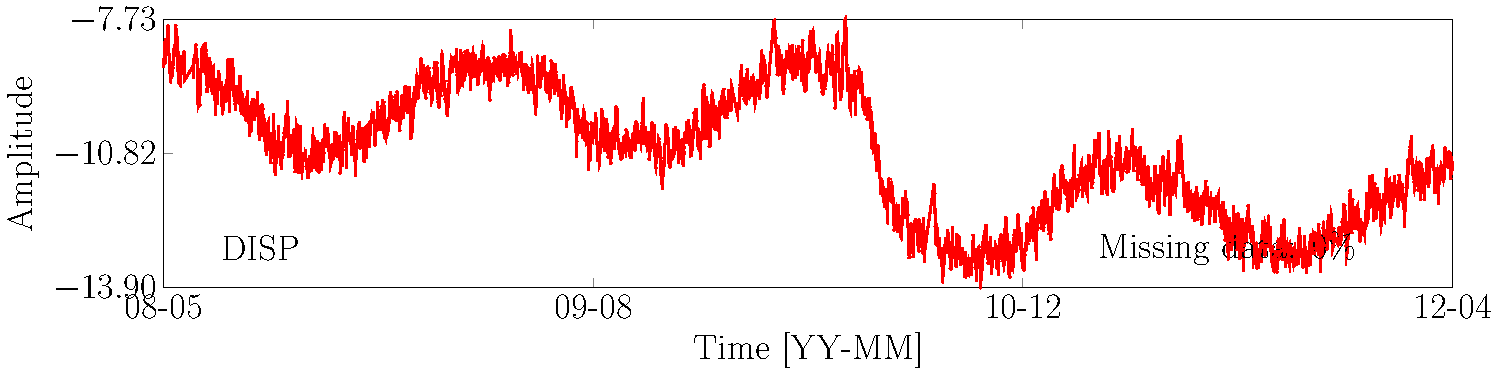
\includegraphics[width=0.95\linewidth]{./docfigs/Example_DISPSIM_ANOMALY/raw/ALL_AMPLITUDES.pdf} 
\caption{Amplitude}
\end{subfigure}
\begin{subfigure}{\linewidth}\centering
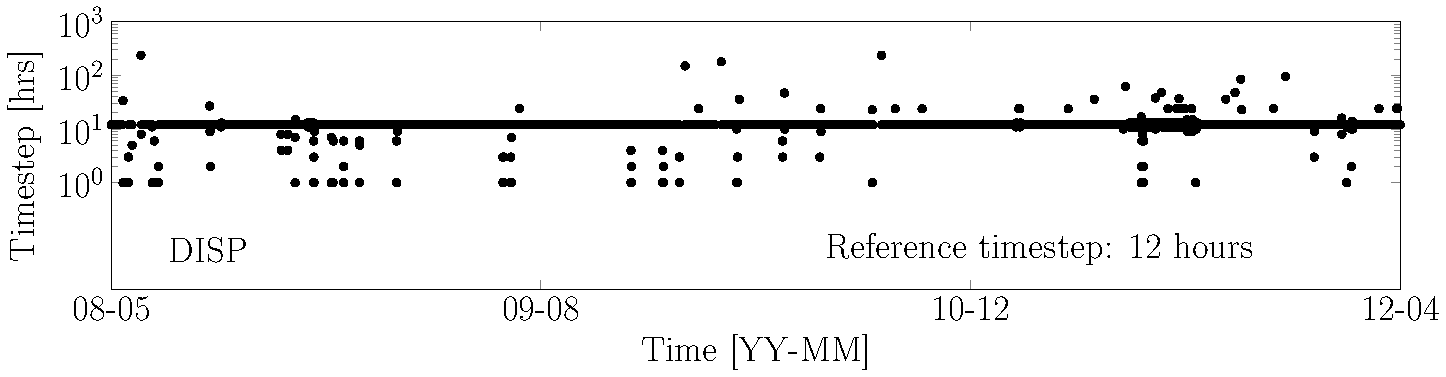
\includegraphics[width=0.9\linewidth]{./docfigs/Example_DISPSIM_ANOMALY/raw/ALL_TIMESTEPS.pdf}
\caption{Timestep}
\end{subfigure}
\begin{subfigure}{\linewidth}\centering
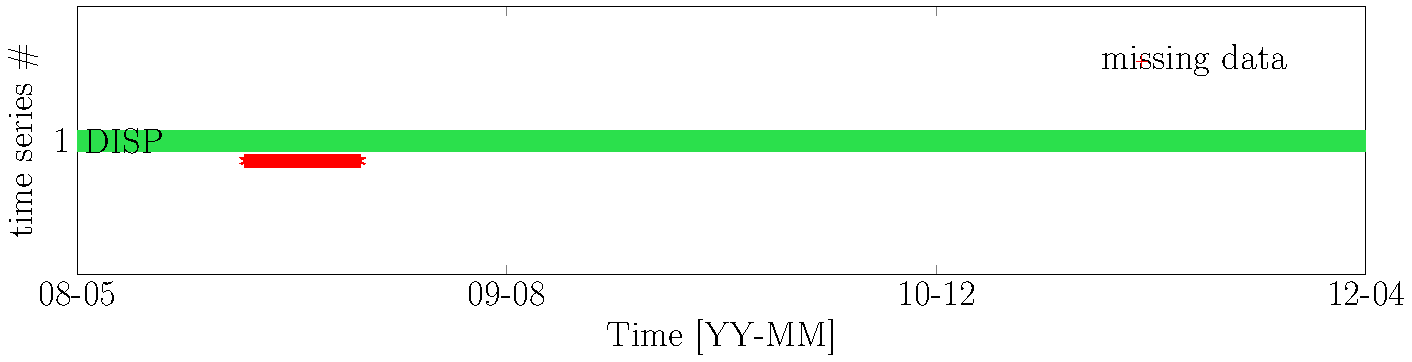
\includegraphics[width=0.9\linewidth]{./docfigs/Example_DISPSIM_ANOMALY/raw/AVAILABILITY.pdf}
\caption{Availability}
\end{subfigure}
\caption{Data used in example \#3}.
\label{fig:DataSummaryRaw3}
\end{figure*}



\subsubsection{Model description}
\label{SS:ModelConstructionExample3}
The model includes two model classes, and the hidden state variables are 
\begin{gather*}
\mathbf{x}^{1}=[x^{\mathtt{L}}, x^{\mathtt{LT}}, x^{\mathtt{LAc}}, x^{\mathtt{P1}\text{,yearly}} , x^{\mathtt{P2}\text{,yearly}}, x^{\mathtt{AR}}]
 \end{gather*}
for the model class \#1, and
\begin{gather*}
\mathbf{x}^{2}=[x^{\mathtt{L}}, x^{\mathtt{LT}}, x^{\mathtt{LA}}, x^{\mathtt{P1}\text{,yearly}} , x^{\mathtt{P2}\text{,yearly}}, x^{\mathtt{AR}}]
 \end{gather*}
for the model class \#2.
The associated model parameters are
\begin{gather*}
\bm\theta=[\sigma_{w}^{\mathtt{TcA},1}, p^{\mathtt{P}, \text{yearly}}, \sigma_{w}^{\mathtt{P}, \text{yearly}}, \phi^{\mathtt{AR}}, \sigma_{w}^{\mathtt{AR}}, \\
 \sigma_{w}^{\mathtt{LA},2}, \sigma_{w}^{\mathtt{TcA}, 21}, \sigma_{w}^{\mathtt{LA}, 11}, \sigma^{1}_{v}, \sigma^{2}_{v}, Z^{11},   Z^{22}] \text{.}
 \end{gather*}
The optimized model parameters values computed using the Newton-Raphson algorithm (see~\ref{SS:THModelParameterEstimation}) with a training period including the entire dataset are
\begin{gather*}
\bm\theta^{\text{*}}=[5\times10^{-8}, 365.2422, 0, 0.72, 0.215, \\
6.6\times10^{-4}, 9.6\times10^{-6}, 0.07 8.85\times10^{-6}, 0.10, 0.08, 0.99995, 0.99963].
\end{gather*}
The estimated initial hidden states mean, covariance,  and model probability values for model class \#1 are 
\begin{align*}
 \bm \mu^{1,\text{*}}_{0} & = [	-9.37 ,	-0.0132	, -7.72\times 10^{-9}	, 1.04  ,	-0.0077	, -0.599    ]^{\intercal}, \text{and} \\
\bm\Sigma^{1,\text{*}}_{0}  & = \text{diag}[	0.124 ,	0.000928,	2.42	,0.000993, 0.00088,	0.32     ],  \text{and} \\
 \pi_{0}^{1,\text{*}} & = 0.998.
\end{align*}
The estimated initial hidden states mean, covariance,  and model probability for model class \#2 are 
\begin{align*}
 \bm \mu^{2,\text{*}}_{0} & = [	-9.49 ,	0.11 ,	-0.063	,  1.04  ,	-0.0077, 	-0.516     ]^{\intercal}, \text{and} \\
 \bm\Sigma^{2,\text{*}}_{0}  & = \text{diag}[	0.614 	,0.49 ,	0.979 ,	0.001,	0.0009	, 0.69    ], \text{and} \\
 \pi_{0}^{2,\text{*}} & = 0.0021.
\end{align*}
The hidden states estimated using the Kalman smoother along with the optimal model parameters and initial hidden states are presented in Figure~\ref{fig:DISPSIMANOMALYOptimizedOptimizedExample3}.


\subsubsection{Run the example from the pre-existing configuration file}
\label{SS:LoadConfigFileEx3}

There is a configuration file CFG\_Example\_DISP\_ANOMALY\_optim.m which is located in the ``config\_files'' folder of the OpenBDLM package.
CFG\_Example\_DISP\_ANOMALY\_optim.m contains the optimized model parameters and initial hidden states values.
There is also a data file DATA\_Example\_DISP\_ANOMALY\_optim.mat that is located in the ``data/mat'' subfolder.
Therefore, it is possible to run the example \#3 by following the steps below while interacting with the \MATLAB{} command line:
\begin{enumerate}
\item Start OpenBDLM. Type \colorbox{light-gray}{\lstinline[basicstyle = \mlttfamily \small, backgroundcolor = \color{light-gray}]!OpenBDLM_main('CFG_Example_DISP_ANOMALY_optim.m');!}.
\item Access hidden states estimation menu. Type \colorbox{light-gray}{\lstinline[basicstyle = \mlttfamily \small, backgroundcolor = \color{light-gray}]!3!}.
\item Run the Kalman smoother to estimate the hidden states. Type \colorbox{light-gray}{\lstinline[basicstyle = \mlttfamily \small, backgroundcolor = \color{light-gray}]!2!}.
\item Save and quit. Type \colorbox{light-gray}{\lstinline[basicstyle = \mlttfamily \small, backgroundcolor = \color{light-gray}]!Q!}.
\end{enumerate}


\subsubsection{Run the example from command line interaction}

The analysis of a new dataset usually requires to start from scratch.
This section explains how to run the example \#3 from scratch, that is, how to load the data presented in Figure~\ref{fig:DataSummaryRaw3}, configure the model, estimate the model parameters and estimate the hidden states.
This may be done by following steps below while interacting with the \MATLAB{} command line:
\begin{enumerate}
\item Start OpenBDLM. Type \colorbox{light-gray}{\lstinline[basicstyle = \mlttfamily \small, backgroundcolor = \color{light-gray}]!OpenBDLM_main;!}.
\item Choose the interactive tool. Type \colorbox{light-gray}{\lstinline[basicstyle = \mlttfamily \small, backgroundcolor = \color{light-gray}]!0!}.
\item Enter the project name. Type \colorbox{light-gray}{\lstinline[basicstyle = \mlttfamily \small, backgroundcolor = \color{light-gray}]!Example_DISP_ANOMALY!}. 
\item Disregard generating synthetic data. Type \colorbox{light-gray}{\lstinline[basicstyle = \mlttfamily \small, backgroundcolor = \color{light-gray}]!no!}. 
\item Load new data. Type \colorbox{light-gray}{\lstinline[basicstyle = \mlttfamily \small, backgroundcolor = \color{light-gray}]!0!}.
\item Select from the graphical user interface the data file Example\_DISP\_ANOMALY\_DISP.csv data file located in the folder `` /data/csv/Example\_DISP\_ANOMALY/''. The Figure~\ref{fig:DataSummaryRaw3} representing the processed data should popup on screen.
\item Save and continue without pre-processing. Type \colorbox{light-gray}{\lstinline[basicstyle = \mlttfamily \small, backgroundcolor = \color{light-gray}]!7!}. The Figure~\ref{fig:DataSummaryRaw3} should popup again on screen.
\item Select the number of model classes. Type \colorbox{light-gray}{\lstinline[basicstyle = \mlttfamily \small, backgroundcolor = \color{light-gray}]!2!}. 
\item Select the model block components for model class \#1. Type \colorbox{light-gray}{\lstinline[basicstyle = \mlttfamily \small, backgroundcolor = \color{light-gray}]![23 31 41]!}.
\item Select the model block components for model class \#2. Type \colorbox{light-gray}{\lstinline[basicstyle = \mlttfamily \small, backgroundcolor = \color{light-gray}]![13 31 41]!}.
\item Select the model parameter constrains. Type \colorbox{light-gray}{\lstinline[basicstyle = \mlttfamily \small, backgroundcolor = \color{light-gray}]![0 1 1]!}\footnote{\lstinline[basicstyle = \mlttfamily \small, backgroundcolor = \color{light-gray}]![0 1 1]! forces the second and third block component (i.e. 31 and 41) to share the same parameters.}.
\item Access model parameter estimation menu. Type \colorbox{light-gray}{\lstinline[basicstyle = \mlttfamily \small, backgroundcolor = \color{light-gray}]!1!}. 
\item Start Newton-Raphson algorithm. Type \colorbox{light-gray}{\lstinline[basicstyle = \mlttfamily \small, backgroundcolor = \color{light-gray}]!1!}. Once the algorithm has converged, the optimized model parameters values should be close to the values presented in Section~\ref{SS:ModelConstructionExample3}. Note that it is possible to get slightly different parameter values\footnote{Keep in mind that the optimization may take several minutes. It is possible to abort the analysis here and to load the configuration file called CFG\_Example\_DISP\_ANOMALY\_optim.m to load pre-computed values of model parameters, as presented in Section~\ref{SS:LoadConfigFileEx3}.}.
\item Estimate the initial hidden states values. Type \colorbox{light-gray}{\lstinline[basicstyle = \mlttfamily \small, backgroundcolor = \color{light-gray}]!2!}.
\item Access hidden states estimation menu. Type \colorbox{light-gray}{\lstinline[basicstyle = \mlttfamily \small, backgroundcolor = \color{light-gray}]!3!}. 
\item Estimate the hidden states using the Kalman smoother. Type \colorbox{light-gray}{\lstinline[basicstyle = \mlttfamily \small, backgroundcolor = \color{light-gray}]!2!}. The estimation should be corresponding to the results presented in Figure~\ref{fig:DISPSIMANOMALYOptimizedOptimizedExample3}.
\item Access export menu. Type \colorbox{light-gray}{\lstinline[basicstyle = \mlttfamily \small, backgroundcolor = \color{light-gray}]!17!}. 
\item Export the current project in a configuration file. Type \colorbox{light-gray}{\lstinline[basicstyle = \mlttfamily \small, backgroundcolor = \color{light-gray}]!1!}.
\item Save and quit OpenBDLM. Type \colorbox{light-gray}{\lstinline[basicstyle = \mlttfamily \small, backgroundcolor = \color{light-gray}]!Q!}.
\end{enumerate}

\begin{figure*}[h!]
\centering
\begin{subfigure}{\linewidth}\centering
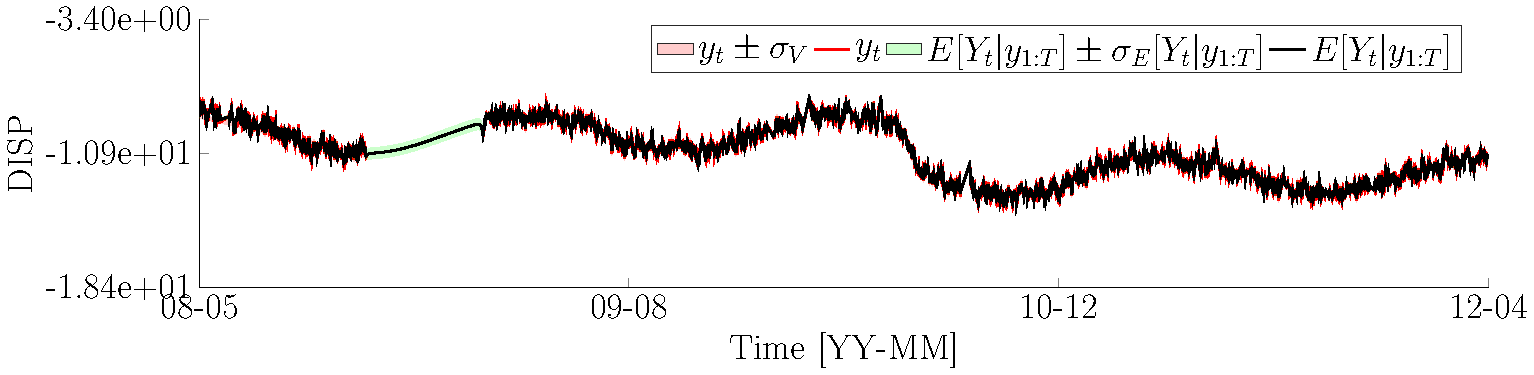
\includegraphics[width=0.9\linewidth]{./docfigs/Example_DISPSIM_ANOMALY/optim_param_optim_initialhiddenstate/DISP_ObservedPredicted.pdf}
\caption{Observed and estimated displacement data}
\end{subfigure}
\begin{subfigure}{\linewidth}\centering
\quad~~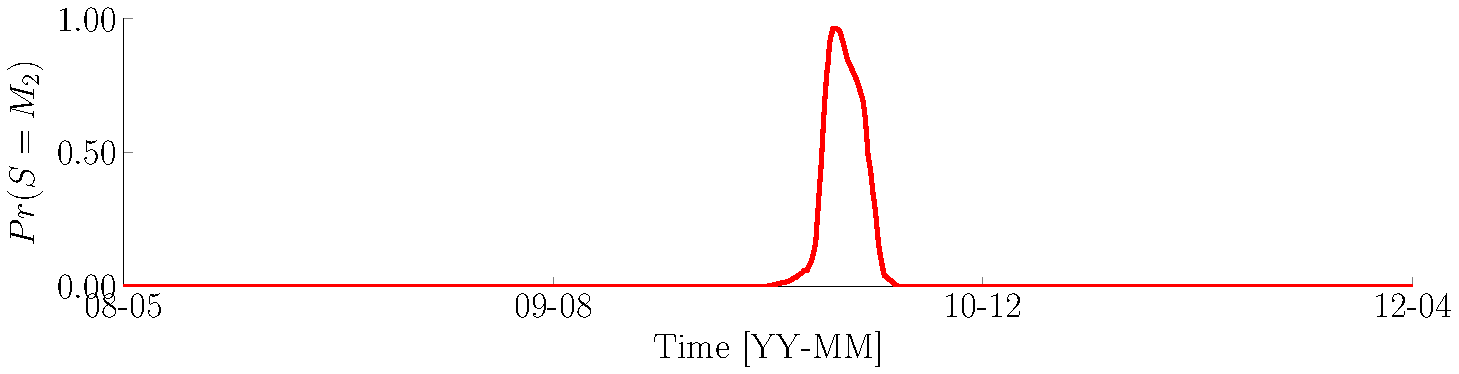
\includegraphics[width=0.85\linewidth]{./docfigs/Example_DISPSIM_ANOMALY/optim_param_optim_initialhiddenstate/ModelProbability.pdf} 
\caption{Estimated probability of anomaly (probability of model class 2)}
\end{subfigure}
\begin{subfigure}{\linewidth}\centering
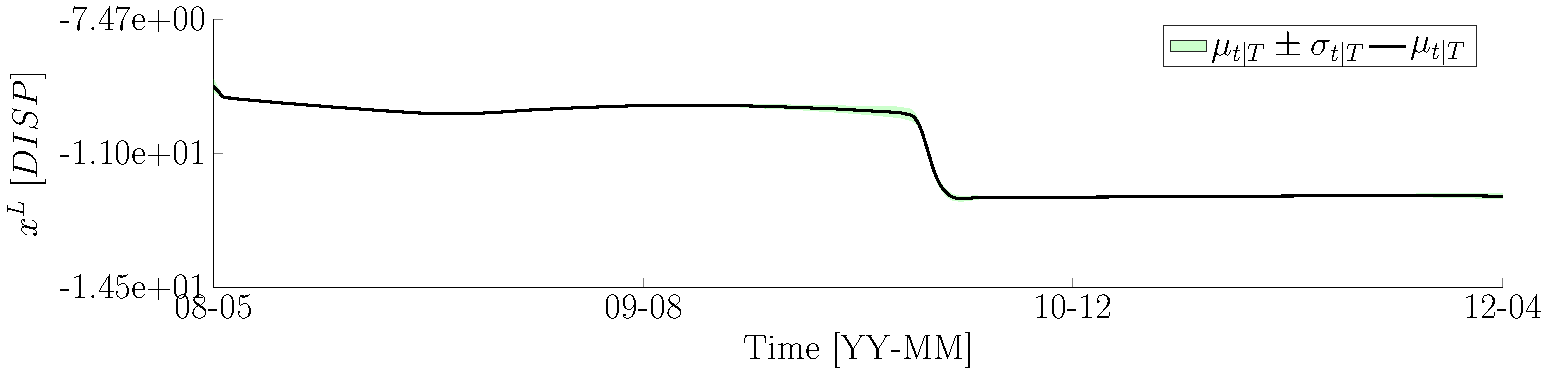
\includegraphics[width=0.9\linewidth]{./docfigs/Example_DISPSIM_ANOMALY/optim_param_optim_initialhiddenstate/DISP_L_1.pdf} 
\caption{Estimated displacement level component}
\end{subfigure}
\begin{subfigure}{\linewidth}\centering
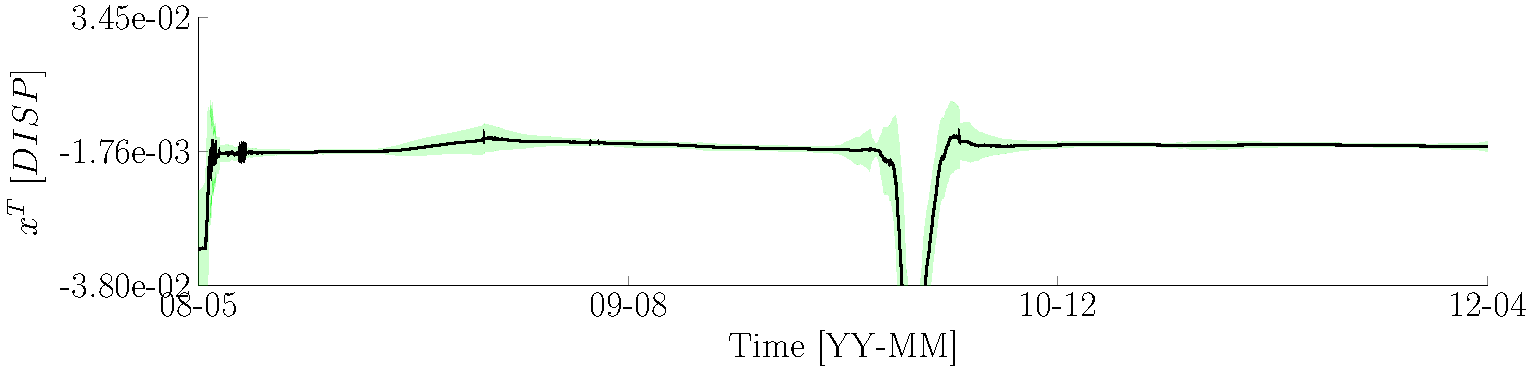
\includegraphics[width=0.9\linewidth]{./docfigs/Example_DISPSIM_ANOMALY/optim_param_optim_initialhiddenstate/DISP_T_2.pdf}
\caption{Estimated displacement local trend component.}
\end{subfigure}
\begin{subfigure}{\linewidth}\centering
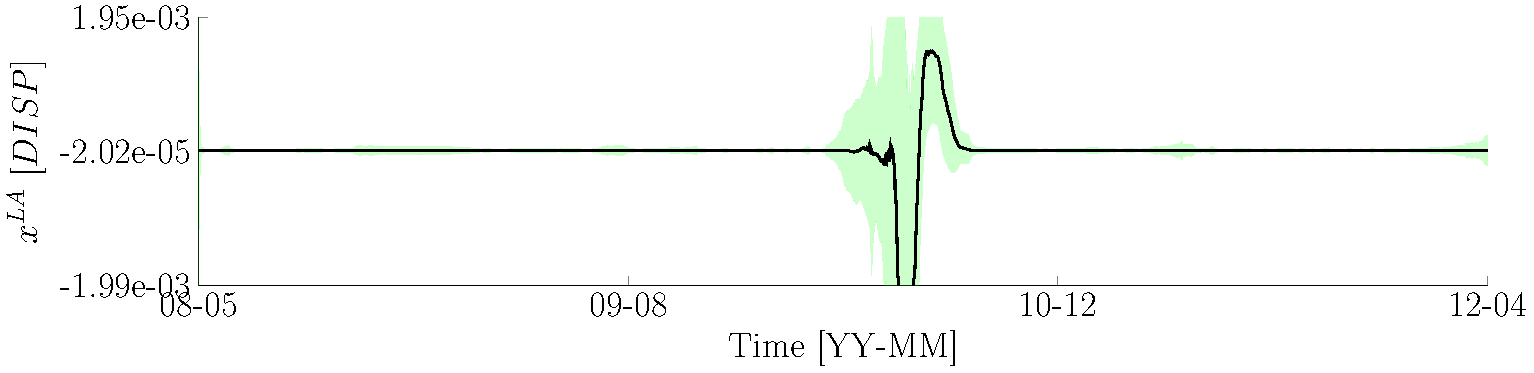
\includegraphics[width=0.9\linewidth]{./docfigs/Example_DISPSIM_ANOMALY/optim_param_optim_initialhiddenstate/DISP_LA_3.pdf}
\caption{Estimated displacement local acceleration component.}
\end{subfigure}
\end{figure*}
\begin{figure*}[htbp]
\ContinuedFloat
\begin{subfigure}{\linewidth}\centering
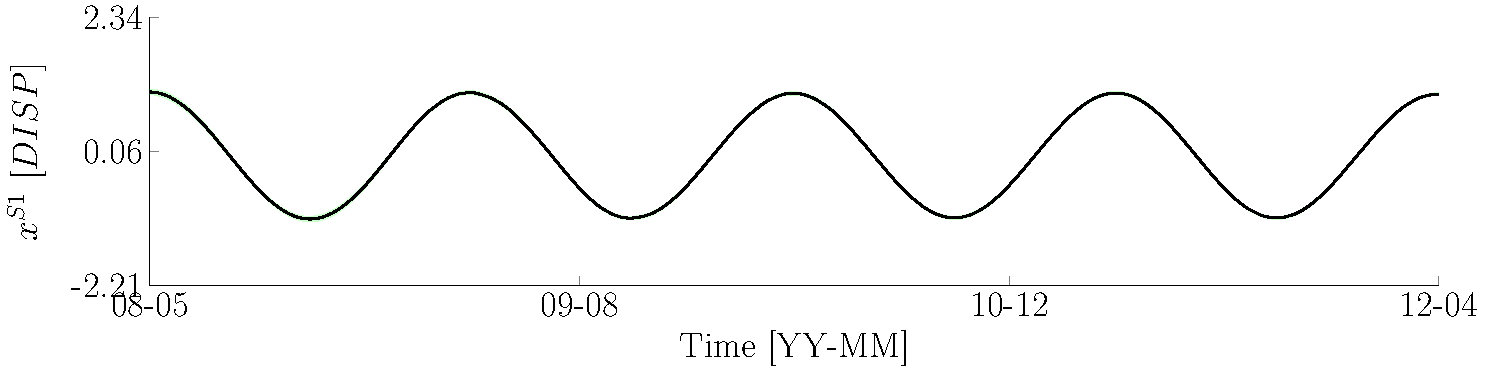
\includegraphics[width=0.9\linewidth]{./docfigs/Example_DISPSIM_ANOMALY/optim_param_optim_initialhiddenstate/DISP_S1_4.pdf}
\caption{Estimated displacement yearly periodic component (first hidden state)}
\end{subfigure}
\begin{subfigure}{\linewidth}\centering
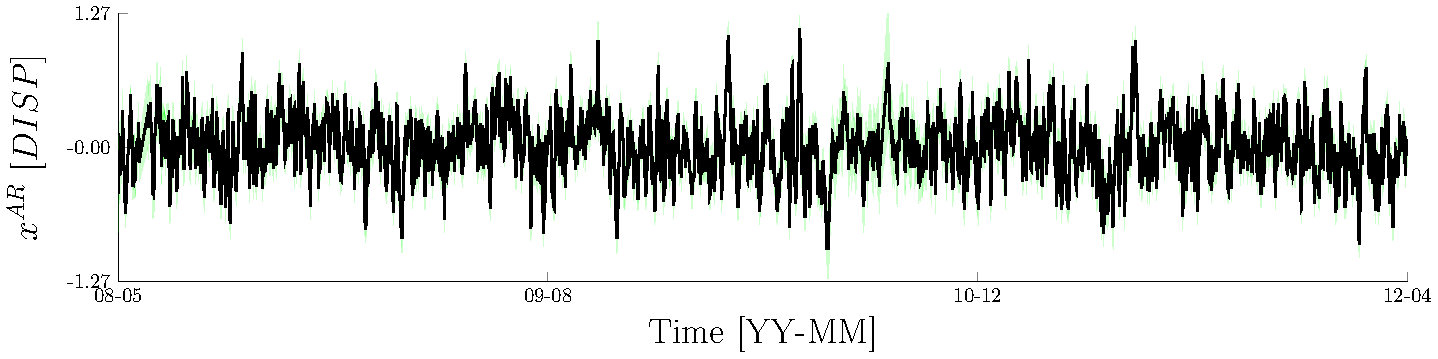
\includegraphics[width=0.9\linewidth]{./docfigs/Example_DISPSIM_ANOMALY/optim_param_optim_initialhiddenstate/DISP_AR_6.pdf} 
\caption{Estimated displacement autoregressive component}
\end{subfigure}
\caption{Estimated results using OpenBDLM with the optimized model parameters and initial hidden states. The hidden states are estimated from the data presented in Figure~\ref{fig:DataSummaryRaw3}a. The solid line and shaded area represent the mean and standard deviation of the estimated hidden states, respectively.}
\label{fig:DISPSIMANOMALYOptimizedOptimizedExample3}
\end{figure*}



